\documentclass[glossy]{beamer}
\useoutertheme{wuerzburg}
\useinnertheme[realshadow,corners=2pt,padding=2pt]{chamfered}
\usecolortheme{shark}
\usepackage[english,serbian]{babel}
\usepackage[utf8]{inputenc} % make weird characters work
\usepackage{tikz}
\newcommand<>{\hover}[1]{\uncover#2{%
 \begin{tikzpicture}[remember picture,overlay]%
 \draw[fill,opacity=0.4] (current page.south west)
 rectangle (current page.north east);
 \node at (current page.center) {#1};
 \end{tikzpicture}}
}


\title{Kratki vodič kroz Git}
\author{Nemanja Radosavljević, Milan Stojković}
\institute{Matematički Fakultet, Univerzitet u Beogradu}
\date{13.5.2016}

\begin{document}

\begin{frame}
\maketitle
\end{frame}




\begin{frame}
\frametitle{Sekcije Git projekta}
\begin{figure}[h!]
\begin{center}
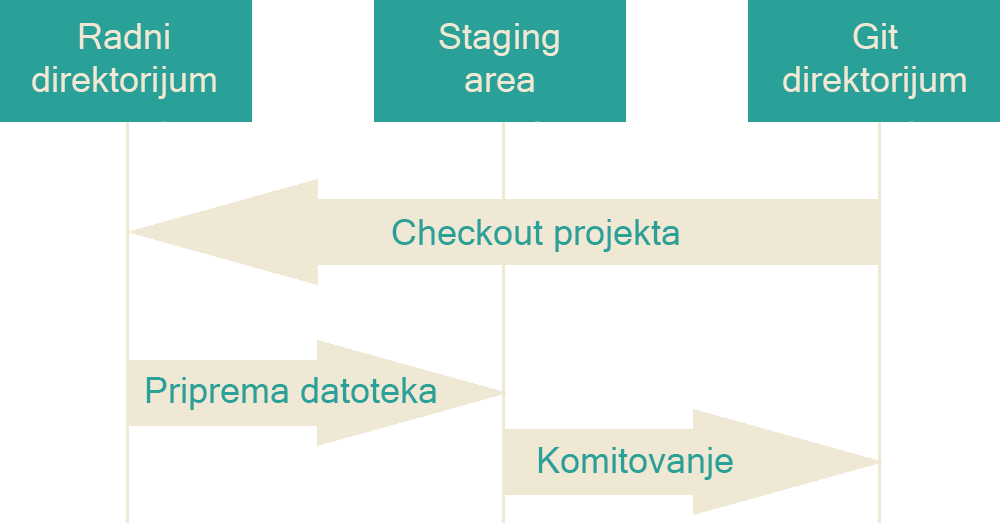
\includegraphics[scale=0.3]{images/sekcije.png}
\end{center}
\end{figure}
\end{frame}





\begin{frame}
\frametitle{Životni ciklus datoteke}
\begin{figure}[h!]
\begin{center}
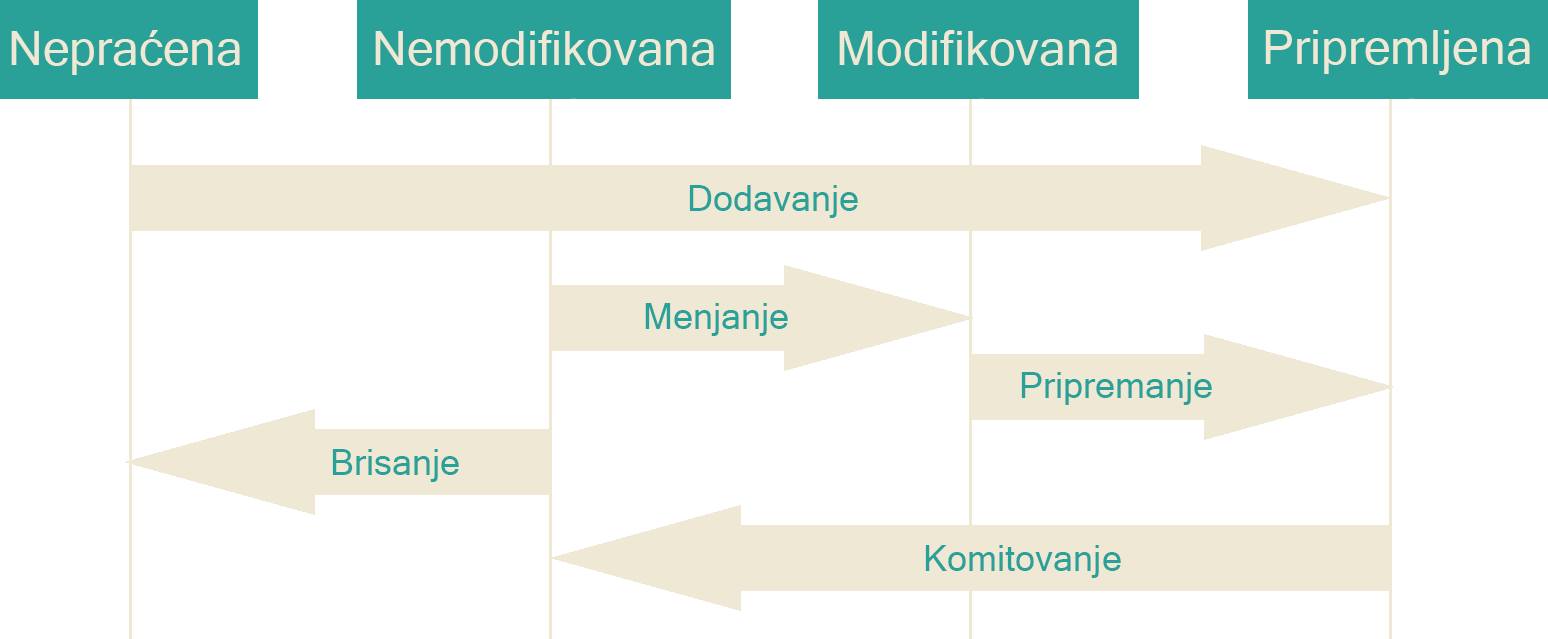
\includegraphics[scale=0.2]{images/lifecycle2.png}
\end{center}
\end{figure}
\end{frame}



\begin{frame}
\frametitle{Predstavljanje i inicijalizacija}
\begin{itemize}
\item $git$ $config --global$ $user.name <name>$
\item $git$ $config --global$ $user.email <email>$
\newline
\item $git$ $init$
\item $git$ $clone$
\end{itemize}
\end{frame}


\begin{frame}
\frametitle{Osnovne komande}
\begin{itemize}
\item $git$ $status$ - provera statusa datoteka
\item $git$ $add$ - dodavanje datoteke u Staging Area
\item $git$ $commit$ - komitovanje pripremljenih datoteka
\item $git$ $log$ - izlistavanje istorije komitova
\item $git$ $checkout$ - prebacivanje sardžaja repozitorijuma u radni direktorijum
\item $git$ $diff$ - prikazivanje razlika između
\begin{itemize}
\item[--] radnog direktorijuma i Staging Area (podrazumevano)
\item[--] radnog direktorijuma i traženog komita (HEAD ili identifikator nekog komita)
\item[--] Staging Area i poslednjeg komita (--cached)
\end{itemize}
\end{itemize}
\end{frame}




\begin{frame}
\frametitle{Ispravljanje grešaka}
\begin{itemize}
\item Lokalne greške

\begin{itemize}
\item[--] $git$ $checkout$
\end{itemize}

\item Greške u Staging Area
\begin{itemize}
\item[--] $git$ $reset$ $HEAD$
\end{itemize}

\item Komitovane greške
\begin{itemize}
\item[--] $git$ $revert <commit>$
\item[--] $git$ $reset <commit> --hard$
\end{itemize}
\end{itemize}
\end{frame}



\begin{frame}
\frametitle{Rad sa granama}
\begin{itemize}
\item Pravljenje grane
\begin{itemize}
\item[--] $git$ $branch <ime>$, praćeno sa $git$ $checkout$
\item[--] $git$ $checkout -b <ime>$
\end{itemize}
\item Prebacivanje na granu
\begin{itemize}
\item[--] $git$ $checkout <ime>$
\end{itemize}
\item Brisanje grane
\begin{itemize}
\item[--] $git$ $branch -d <ime>$
\end{itemize}


\end{itemize}
\end{frame}

\begin{frame}
\frametitle{This is a slide}
\begin{itemize}
\item These are more points
\item These are more points
\item These are more points
\item These are more points
\item These are more points
\end{itemize}
\end{frame}




\begin{frame}
 \frametitle{A frame}
 Some text
 \hover<2>{
  \begin{minipage}{0.8\linewidth}
   \begin{block}{Hvala na pažnji!}
  	ovde jos nesto
   \end{block}
  \end{minipage}
 }
\end{frame}

\end{document}